\documentclass[10pt,a4paper]{article}
\usepackage[margin=2.0cm]{geometry}
\usepackage{graphicx,booktabs,amsmath,siunitx,caption,subcaption,hyperref,xcolor}
\graphicspath{{../figures/}}
\captionsetup{font=small,labelfont=bf}
\sisetup{detect-all}
\hypersetup{colorlinks=true,linkcolor=blue!50!black,urlcolor=blue!50!black,citecolor=blue!50!black}
\setlength{\parskip}{3pt}

\title{\textbf{Conjugate Heat Transfer Analysis and Design Optimisation of a Microchannel Cold Plate for High-Power AI Processors}}
\author{Chanduri Sreekrishna Abhay\\\small B.Tech.\ Aeronautical Engineering, Jain (Deemed-to-be University), Bengaluru\\\small\url{https://github.com/KrishnaChanduri06/microchannel-cold-plate-cht}}
\newcommand{\qeff}{q^{\prime\prime}_\mathrm{eff}}
\newcommand{\qbot}{q^{\prime\prime}_\mathrm{bot}}
\date{October 2026}

\begin{document}
\maketitle

\begin{abstract}
\noindent A three-dimensional conjugate heat transfer (CHT) model of a single-phase copper microchannel heat sink was built in Ansys Fluent 2026~R1, scripted in Python (PyFluent) with a structured hexahedral mesh generator, and validated against the experiments of Qu and Mudawar (2002). Across six operating points ($Re = 226$--$1454$, $\qeff = 100$ and \SI{200}{W/cm^2}) the CFD predicts the thermocouple temperatures with a mean error of 5.4\,\%, matching the original authors' CFD (5.6\,\%), and closes the energy balance within 1.5\,\%. A three-mesh Grid Convergence Index study gives discretisation uncertainties below 4.6\,\%, and a no-heating case Richardson-extrapolates to within 0.1\,\% of the analytical laminar developing-flow pressure drop. A 1-D resistance-network model with a fully developed three-wall Nusselt number (computed here as 5.30) over-predicts temperatures by up to 62\,\%; the error is governed almost entirely by the ratio of thermal entry length to channel length. The validated model was then used for an automated 36-case design study of a product-like cold plate (\SI{30}{\celsius} water, \SI{100}{W/cm^2}): narrow channels with thin fins dominate the thermal-resistance/pumping-power Pareto front, and silicon is 15--35\,\% worse than copper at identical geometry. A multi-channel Ansys Icepak model confirms that the base temperature is uniform across the plate width, supporting the unit-cell assumption.
\end{abstract}

\section{Introduction}
Data-centre AI accelerators now dissipate around \SI{1}{kW} per package at average die fluxes near \SI{100}{W/cm^2}, beyond the reach of air cooling. Liquid cold plates with microchannels are the established solution, and channels embedded in the die are under active research. This work builds and validates a CHT model of a classic benchmark microchannel heat sink \cite{qu2002}, quantifies where simple correlation-based sizing fails, and uses the validated model to explore cold-plate design trade-offs.

\section{Benchmark and models}
\subsection{Benchmark}
Qu and Mudawar \cite{qu2002} tested an oxygen-free copper heat sink with 21 channels of \SI{231}{\micro m}\,$\times$\,\SI{713}{\micro m} cross-section and \SI{44.764}{mm} length, closed by a polycarbonate cover, cooled by \SI{15}{\celsius} water at $Re = 139$--$1672$, and heated with $\qeff = 100$ and \SI{200}{W/cm^2} over a $1.0\times\SI{4.48}{cm^2}$ planform. Four thermocouples sit \SI{3.175}{mm} above the heated surface. Figures 4--7 of the paper were digitised automatically (marker detection and curve tracing with OpenCV, calibrated against the axis ticks); the three figures that share flow rates agree in $Re$ to 0.2\,\%.

\subsection{1-D analytical model}
Friction uses the Shah \& London fully developed $fRe = 17.2$ ($\alpha = 0.324$) plus the Hagenbach entrance factor $K(\infty) = 1.18$ \cite{shah1978}. Because the cover is almost adiabatic only three walls are heated; the corresponding fully developed H1 Nusselt number was computed with a 2-D finite-volume solver, giving $Nu_3 = 5.30$ (the solver reproduces the four-wall values 3.608, 4.124, 5.333 to $\pm 0.002$). Fins have efficiency $\eta_f = \tanh(mH)/(mH) \approx 0.97$, and conduction, convection and caloric resistances are combined in series. Re uses inlet properties as in the paper; $\Delta P$ and $h$ use mean-bulk properties.

\subsection{CFD model}
The unit cell (one channel, two half fins, copper base, cover, and the three \SI{1.6}{mm} air slots of the test section, Fig.~\ref{fig:fields}) is meshed with a structured hexahedral mesh generator that writes Fluent's native \texttt{.msh} format (orthogonal quality 1.0; baseline 89\,760 cells, clustered at walls and inlet). The flow is steady and laminar; water $\mu(T)$, $k(T)$ and $c_p(T)$ are polynomial fits to CoolProp (max error 0.06\,\%); density is constant. Boundary conditions follow the paper: uniform inlet velocity at \SI{15}{\celsius}, zero-gauge outlet, a uniform heat flux on the copper part of the base ($\qbot = P_W/(NA_\mathrm{bot}) = \SI{114.3}{W/cm^2}$ at the nominal 100), $h = \SI{10}{W/m^2K}$ on the cover top, and symmetry sides. The pressure-based coupled solver with second-order schemes is iterated until the thermocouple temperatures change by less than \SI{0.005}{K} and $\Delta P$ by less than 0.01\,\% per 100 iterations (about 500 iterations, 90\,s per case on 4 cores).

\section{Verification}
\begin{table}[h]\centering\small
\caption{Grid Convergence Index \cite{celik2008} at \SI{100}{W/cm^2}, $Re = 890$ (meshes of 29\,820 / 89\,760 / 297\,891 cells, $r \approx 1.5$).}\label{tab:gci}
\begin{tabular}{lcccccc}\toprule
Quantity & coarse & medium & fine & extrapolated & $p$ & GCI$_\mathrm{fine}$\\\midrule
$\Delta P_\mathrm{ch}$ [bar] & 0.325 & 0.334 & 0.338 & 0.341 & 2.3 & 1.0\,\%\\
$T_\mathrm{heater,avg}-T_\mathrm{in}$ [K] & 42.42 & 42.47 & 42.71 & 42.77 & 3.8 & 0.2\,\%\\
$T_\mathrm{heater,max}-T_\mathrm{in}$ [K] & 50.07 & 50.66 & 51.12 & 52.12 & 0.9 & 2.4\,\%\\
$T_\mathrm{TC3}-T_\mathrm{in}$ [K] & 36.16 & 36.61 & 36.99 & 38.37 & 0.6 & 4.6\,\%\\
$\Delta P_\mathrm{ch}$, no heating [bar] & 0.415 & 0.442 & 0.455 & \textbf{0.467} & 1.9 & 3.3\,\%\\\bottomrule
\end{tabular}\end{table}

All quantities are mesh-converged to within 5\,\% on the baseline mesh (Table~\ref{tab:gci}). For the no-heating case the laminar developing-flow pressure drop is known analytically, $[4fL/D_h + K(\infty)]\,\rho u^2/2 = \SI{0.4678}{bar}$; the Richardson-extrapolated CFD value of \SI{0.4672}{bar} agrees within 0.1\,\%, with observed order 1.9, which verifies the solver set-up, boundary conditions and mesh writer.

\section{Validation}
\begin{figure}[t]\centering
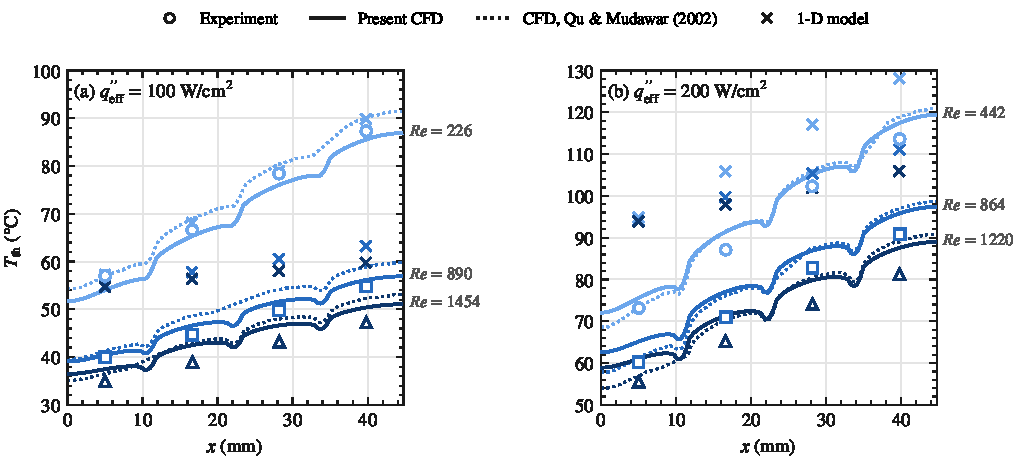
\includegraphics[width=\linewidth]{tc_line_validation.pdf}
\caption{Temperature along the thermocouple line: experiment (open markers), present CFD (solid), CFD of Qu and Mudawar (dotted) and the 1-D model at the thermocouple positions ($\times$). The dips mark the three air slots.}\label{fig:tcline}
\end{figure}

\begin{table}[h]\centering\small
\caption{Mean absolute error against the experiment at the six validation points.}\label{tab:val}
\begin{tabular}{lccc}\toprule
Quantity & present CFD & Qu \& Mudawar CFD & 1-D model\\\midrule
Thermocouple temperature, Fig.~7 & \textbf{5.4\,\%} & 5.6\,\% & 28.5\,\%\\
Thermocouple rise $T_\mathrm{tc}-T_\mathrm{in}$, Fig.~6 & \textbf{7.2\,\%} & -- & 40.5\,\%\\
Water temperature rise, Fig.~5 & 1.5\,\% & -- & 1.5\,\%\\
Channel pressure drop, Fig.~4b & 10.5\,\% & 18.8\,\%$^\dagger$ & 35\,\%\\\bottomrule
\multicolumn{4}{l}{\footnotesize $^\dagger$ includes their plenum contraction/expansion losses.}
\end{tabular}\end{table}

The present CFD reproduces the measured temperature distribution as closely as the published CFD and follows it point by point, including the slot dips (Fig.~\ref{fig:tcline}, Table~\ref{tab:val}). The residual 5--12\,\% warm bias grows with $Re$ in both CFD studies; plausible causes are thermocouple contact and lead conduction, which normally make thermocouples read low, the unspecified slot height, and the less-than-1\,\% heat loss. \begin{figure}[t]\centering
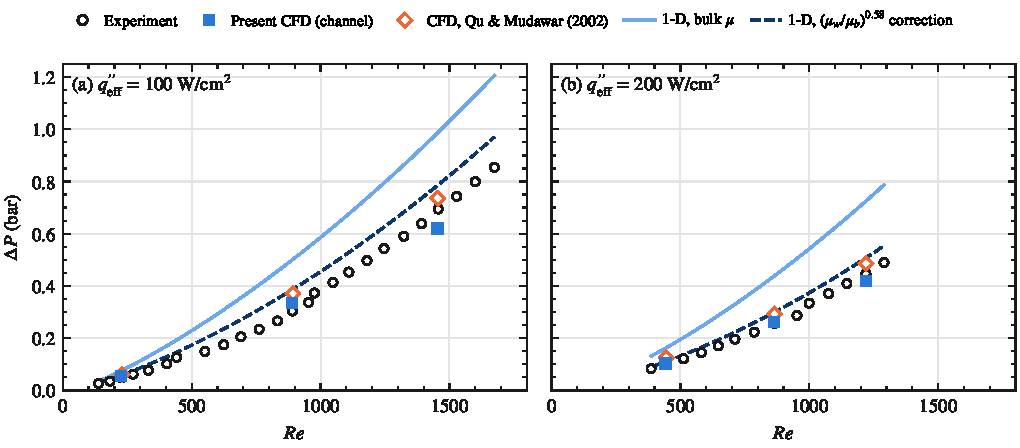
\includegraphics[width=\linewidth]{pressure_drop.pdf}
\caption{Pressure drop: experiment, present CFD (channel only), CFD of Qu and Mudawar (including plenum losses) and the 1-D model with bulk viscosity and with the wall-viscosity correction.}\label{fig:dp}
\end{figure}
The measured $\Delta P$ (Fig.~\ref{fig:dp}) includes plenum losses that are not geometrically specified; adding one velocity head of loss to the CFD channel value raises the error to 24\,\%, which suggests strong pressure recovery in the outlet plenum. Heating reduces $\Delta P$ markedly (\SI{0.44}{bar} cold vs \SI{0.33}{bar} heated at $Re = 890$) because the hot walls lower the near-wall viscosity, which is the main reason bulk-property correlations over-predict it; a $(\mu_w/\mu_b)^{0.58}$ correction \cite{kakacyener1994} cuts the 1-D over-prediction from 56--65\,\% to 13--21\,\%.

\section{Why the 1-D model fails: thermal development}
\begin{figure}[t]\centering
\begin{subfigure}{0.49\linewidth}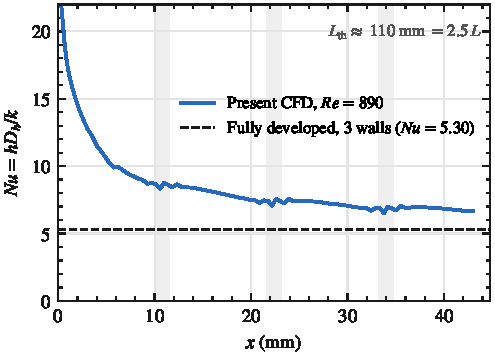
\includegraphics[width=\linewidth]{local_nusselt.pdf}\caption{}\end{subfigure}
\begin{subfigure}{0.49\linewidth}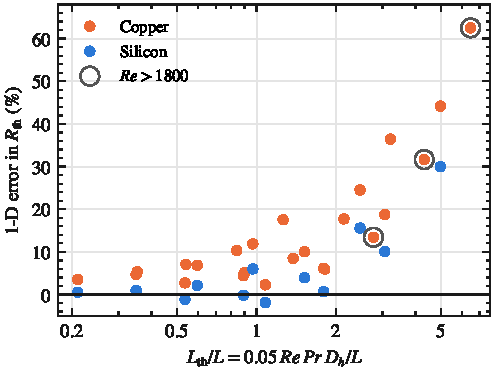
\includegraphics[width=\linewidth]{error_vs_entry_length.pdf}\caption{}\end{subfigure}
\caption{(a) Local Nusselt number from CFD along the channel at $Re = 890$ (shaded: air slots) against the fully developed three-wall value. (b) 1-D thermal-resistance error vs CFD across the design study, against the thermal entry length ratio.}\label{fig:nu}
\end{figure}
At $Re = 890$ the thermal entry length $L_\mathrm{th} = 0.05\,Re\,Pr\,D_h \approx \SI{110}{mm}$ is 2.5 times the channel length, so the boundary layer never becomes fully developed: the CFD local Nusselt number falls from above 20 at the inlet to about 7 at the outlet, with a channel mean of 9.0, which is 1.7 times the fully developed 5.30 (Fig.~\ref{fig:nu}a). The fully developed 1-D model therefore over-predicts temperatures most at high $Re$ and near the inlet (TC1). Across the design study (Fig.~\ref{fig:nu}b) the 1-D error is 0--7\,\% for $L_\mathrm{th}/L < 1$ and rises to 30--62\,\% for $L_\mathrm{th}/L > 3$. Fully developed correlations are adequate for sizing while the thermal entry length is shorter than the channel, and beyond that CFD or developing-flow correlations are needed.

\section{Design study}
\begin{figure}[t]\centering
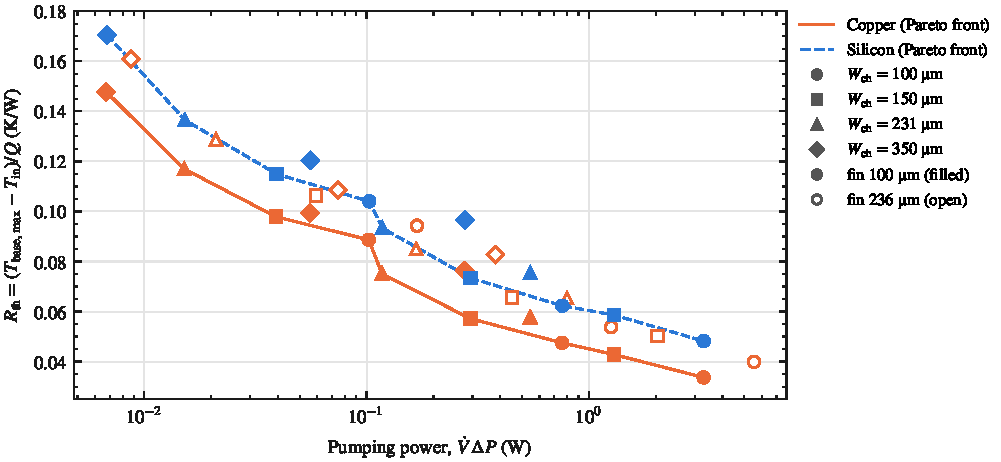
\includegraphics[width=\linewidth]{pareto.pdf}
\caption{Thermal resistance against channel pumping power for the design study at \SI{100}{W/cm^2} (\SI{448}{W}, \SI{30}{\celsius} water). Marker shape: channel width; filled: \SI{100}{\micro m} fins, open: \SI{236}{\micro m} fins; lines: Pareto fronts.}\label{fig:pareto}
\end{figure}
A product-like plate was studied: a \SI{1}{mm} base, a \SI{1}{mm} lid of the same metal (so all four channel walls carry heat), no slots, \SI{30}{\celsius} inlet water and a uniform \SI{100}{W/cm^2} over the $1\times\SI{4.48}{cm^2}$ footprint. A PyFluent driver swept channel width (100--\SI{350}{\micro m}), fin width (100, \SI{236}{\micro m}), total flow (200--\SI{1000}{ml/min}) and solid (copper, silicon), 36 cases with energy balances of 0.999--1.000. The figure of merit is $R_\mathrm{th} = (T_\mathrm{base,max}-T_\mathrm{in})/Q$.
\begin{itemize}\setlength\itemsep{1pt}
\item \textbf{Thin fins and narrow channels form the whole Pareto front} (Fig.~\ref{fig:pareto}): a smaller $D_h$ raises $h$ and the finer pitch adds wetted area, cutting the dominant convective resistance, at the cost of $\Delta P$. The best copper design (\SI{100}{\micro m}/\SI{100}{\micro m}, \SI{1000}{ml/min}) reaches \SI{0.034}{K/W}, a \SI{45}{\celsius} base at \SI{448}{W}, for \SI{3.3}{W} of pumping power. A design near the knee (\SI{150}{\micro m}/\SI{100}{\micro m}, \SI{500}{ml/min}) needs ten times less pumping power for 1.7 times the resistance.
\item \textbf{Silicon is 15--35\,\% worse than copper} at identical geometry ($\eta_f$ 0.68--0.89 vs 0.84--0.96). Silicon microchannels pay off only when they are etched into the die \cite{vanerp2020}, eliminating the thermal interface material, whose resistance typically exceeds this penalty.
\item \textbf{At \SI{200}{W/cm^2}} $R_\mathrm{th}$ changes by less than 1.2\,\% (thermally linear) while $\Delta P$ falls 9--14\,\% (lower viscosity). Copper Pareto designs keep the base at or below \SI{81}{\celsius}; the silicon knee design reaches \SI{95}{\celsius}.
\item Four high-flow cases with thick fins or wide channels have inlet $Re = 1860$--$2300$, near laminar transition; none is Pareto-optimal.
\end{itemize}

\section{Multi-channel Icepak model}
To test the unit-cell assumption the heat sink was also modelled in Ansys Icepak (AEDT 2025~R2, scripted with PyAEDT): channels, fins, thicker edge walls, slots and cover, with constant water properties at the mean bulk temperature. Resolving the flow in the \SI{0.231}{mm} channels beside thin fins required cells of about \SI{0.03}{mm} across and through the channels; coarser meshes closed the channels. At that resolution the full 21-channel plate needs 3.1\,M cells, above the Student licence limit, so a 7-channel strip with the same pitch and edge walls was solved instead. The base temperature under the outermost channel equals the centre value to \SI{0.01}{K} (\SI{72.66}{\celsius} both), which confirms that copper spreading makes the unit-cell idealisation sound for the solid, although the edge channel's water runs warmer because it also absorbs the heat of the thicker side wall. Absolute temperatures are 7--\SI{15}{K} above the validated Fluent model, worst near the inlet: Icepak's uniform cut-cell mesh (\SI{0.25}{mm} axial cells, no wall clustering) under-resolves the thin entrance boundary layer that dominates heat transfer there. For microchannels a structured, wall-clustered mesh is considerably more effective than a larger uniform mesh.

\section{Conclusions}
\begin{enumerate}\setlength\itemsep{1pt}
\item A scripted Fluent CHT workflow (structured hexahedral mesher, PyFluent driver) reproduces the Qu \& Mudawar experiments with 5.4\,\% mean temperature error, equal to the original CFD, and verifies against analytical theory to 0.1\,\%.
\item Fully developed 1-D models over-predict microchannel temperatures by up to 62\,\% because the flow is thermally developing; the error scales with $L_\mathrm{th}/L$, which gives a simple validity criterion.
\item For a \SI{100}{W/cm^2} AI-class cold plate, narrow channels with thin fins dominate the $R_\mathrm{th}$--pumping-power trade-off; copper beats silicon by 15--35\,\% unless the silicon removes the interface layer.
\end{enumerate}
\textbf{Limitations and next steps:} the chip stack and thermal interface are not modelled, the inlet and outlet plenums are excluded, and only straight channels were studied. Natural extensions are manifold microchannels, non-uniform hotspot heating, and a physical test rig.

\begin{thebibliography}{9}\small
\bibitem{qu2002} W.~Qu, I.~Mudawar, Experimental and numerical study of pressure drop and heat transfer in a single-phase micro-channel heat sink, \emph{Int.\ J.\ Heat Mass Transfer} 45 (2002) 2549--2565.
\bibitem{shah1978} R.~K.~Shah, A.~L.~London, \emph{Laminar Flow Forced Convection in Ducts}, Academic Press, 1978.
\bibitem{celik2008} I.~B.~Celik et al., Procedure for estimation and reporting of uncertainty due to discretization in CFD applications, \emph{J.\ Fluids Eng.} 130 (2008) 078001.
\bibitem{kakacyener1994} S.~Kaka\c{c}, Y.~Yener, \emph{Convective Heat Transfer}, 2nd ed., CRC Press, 1994, Eq.~(9.34b).
\bibitem{vanerp2020} R.~van~Erp, R.~Soleimanzadeh, L.~Nela, G.~Kampitsis, E.~Matioli, Co-designing electronics with microfluidics for more sustainable cooling, \emph{Nature} 585 (2020) 211--216.
\end{thebibliography}

\appendix
\section{Field results}
\begin{figure}[h]\centering
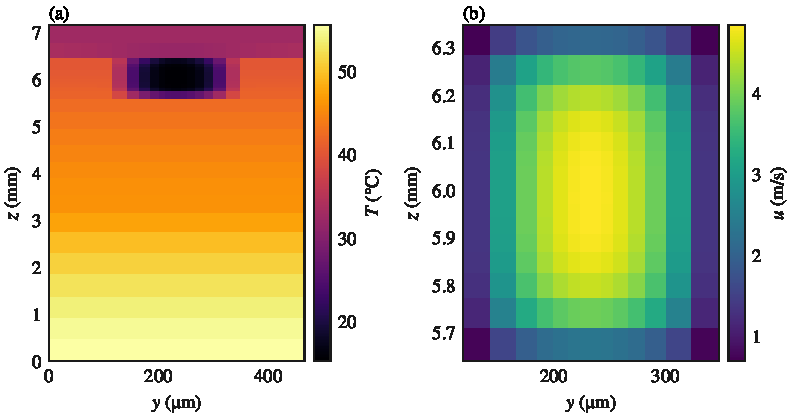
\includegraphics[width=0.7\linewidth]{cross_section.pdf}\\[4pt]
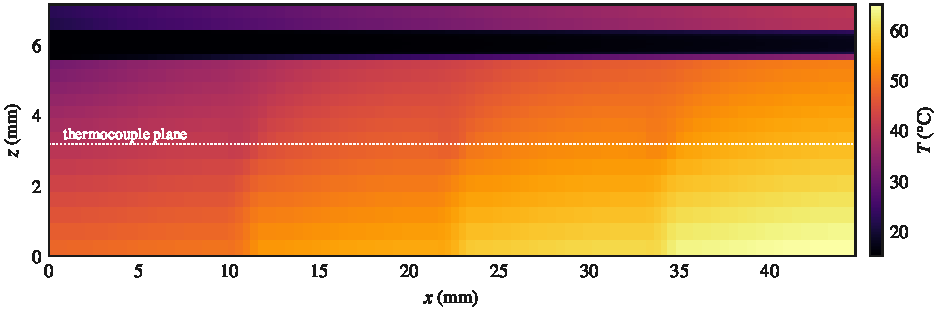
\includegraphics[width=\linewidth]{midplane_temperature.pdf}
\caption{CFD solution at \SI{100}{W/cm^2}, $Re = 890$. Top: cross-section at mid-length, (a) temperature and (b) axial velocity. Bottom: temperature on the channel mid-plane; the steps in the base are at the three air slots.}\label{fig:fields}
\end{figure}
\end{document}
